\section{Results}
\label{s:results}
%Results; this should be a readable summary of the results from applying the approach. Don’t pursue death by figures but carefully select what visualizations (figures, tables) are functional for telling your story and logically lead to the main conclusions and policy advice?

% Convincing story, consistent with approach using carefully designed visuals and tables to support narrative

\subsection{Uncertainty Analysis}



\subsection{Robust Decision Making}
%Look at the policies for the five different scenarios, and examine tradeoffs using different robustness metrics.
For the robust decision making process two metrics were used: Satisficing and maximum regret. The robustness metrics are discussed below for the three different actors.\newline

The threshold values for the satisficing analysis can be found in \autoref{tab:threshold}. The threshold values for the total costs are the exact budgets of the institutions for water/traffic management so that it is a somewhat realistic representation. Expected annual damage was taken as 10\% of the Total costs that are available every year to the institutions. The values for expected annual casualties is calculated from the maximum risk of 1:100,000 people that can die from flooding multiplied \cite{slootjesandvandermost_2016} . Which is then multiplied with the amount of inhabitants of the area.
% Please add the following required packages to your document preamble:

\begin{table}[H]
\centering
\caption{This table shows the threshold values for the three actors. The values for the town of Gorssel come from its bigger municipality Lochem \cite{gorssel-2021}. Deventers value is derived from \cite{deventer-2021}. The value for Overijssel is gained from \cite{provincie-overijssel-2021}.}
\label{tab:threshold}
\begin{tabular}{@{}llll@{}}
\cmidrule(l){2-4}
 &
  \multicolumn{3}{c}{\textbf{Robustness threshold values}} \\ \cmidrule(l){2-4} 
\multicolumn{1}{l|}{} &
  \multicolumn{1}{l|}{\textbf{Outcome}} &
  \multicolumn{1}{l|}{\textbf{Goal}} &
  \multicolumn{1}{l|}{\textbf{Threshold}} \\ \cmidrule(l){2-4} 
\multicolumn{1}{c|}{\multirow{3}{*}{Gorssel}} &
  \multicolumn{1}{l|}{\begin{tabular}[c]{@{}l@{}}Expected annual\\ damage\end{tabular}} &
  \multicolumn{1}{l|}{Minimize} &
  \multicolumn{1}{l|}{$5.4E+05$} \\ \cmidrule(l){2-4} 
\multicolumn{1}{c|}{} &
  \multicolumn{1}{l|}{\begin{tabular}[c]{@{}l@{}}Expected annual\\ casualties\end{tabular}} &
  \multicolumn{1}{l|}{Minimize} &
  \multicolumn{1}{l|}{$1.0E-05$} \\ \cmidrule(l){2-4} 
\multicolumn{1}{c|}{} &
  \multicolumn{1}{l|}{Total costs} &
  \multicolumn{1}{l|}{Minimize} &
  \multicolumn{1}{l|}{$5.4E+06$} \\ \cmidrule(l){2-4} 
\multicolumn{4}{l}{} \\ \cmidrule(l){2-4} 
\multicolumn{1}{l|}{\multirow{3}{*}{Deventer}} &
  \multicolumn{1}{l|}{\begin{tabular}[c]{@{}l@{}}Expected annual\\ damage\end{tabular}} &
  \multicolumn{1}{l|}{Minimize} &
  \multicolumn{1}{l|}{$1.1E+06$} \\ \cmidrule(l){2-4} 
\multicolumn{1}{l|}{} &
  \multicolumn{1}{l|}{\begin{tabular}[c]{@{}l@{}}Expected annual\\ casualties\end{tabular}} &
  \multicolumn{1}{l|}{Minimize} &
  \multicolumn{1}{l|}{$1.0E-05$} \\ \cmidrule(l){2-4} 
\multicolumn{1}{l|}{} &
  \multicolumn{1}{l|}{Total costs} &
  \multicolumn{1}{l|}{Minimize} &
  \multicolumn{1}{l|}{$1.1E+07$} \\ \cmidrule(l){2-4} 
\multicolumn{4}{l}{} \\ \cmidrule(l){2-4} 
\multicolumn{1}{l|}{\multirow{3}{*}{Overijssel}} &
  \multicolumn{1}{l|}{\begin{tabular}[c]{@{}l@{}}Expected annual\\ damage\end{tabular}} &
  \multicolumn{1}{l|}{Minimize} &
  \multicolumn{1}{l|}{$1.53E+06$} \\ \cmidrule(l){2-4} 
\multicolumn{1}{l|}{} &
  \multicolumn{1}{l|}{\begin{tabular}[c]{@{}l@{}}Expected annual\\ casualties\end{tabular}} &
  \multicolumn{1}{l|}{Minimize} &
  \multicolumn{1}{l|}{$1.0E-05$} \\ \cmidrule(l){2-4} 
\multicolumn{1}{l|}{} &
  \multicolumn{1}{l|}{Total costs} &
  \multicolumn{1}{l|}{Minimize} &
  \multicolumn{1}{l|}{$1.53E+07$} \\ \cmidrule(l){2-4} 
\end{tabular}
\end{table}
%#################################################################
%   REGRET AND SATISFICING - GORSSEL
%#################################################################
\subsubsection{Gorssel}
\textbf{Satisficing results} \newline
The results from this analysis: The results for Gorssels satisficing analysis with the domain criterion are shown in \autoref{fig:domain_criterion_gorssel}. The graph shows that there are several policies that 
Gorssel only has regret for their total costs, but this regret is negative, so ?
Gorssel has several policies that come above the now set threshold. These three policies results show no damage or loss of life for Gorssel, shown in Table \ref{tab:Gorssel}. Two of them have the same total costs, and one of them is free? Which makes it a tad weird. 

\textbf{results shown in figures: still have to add the tables which show the policy that is satisficing for every threshold. Also I'll put it nicely tomorrow. }
\begin{itemize}
    \item Gorssel has 27 policies of which in the end only 1 is satisficing for every threshold. This policy is : ....
    \item Gorsse has uncertainty about the total costs that they'll have.
    \item The policies generated for Gorssel show that their policies have high treadeoffs between either deatsh and damages vs total costs. This makes it more difficult to find good policy options. 
\end{itemize}

\begin{figure}[H]
  \centering
  \begin{minipage}[b]{0.4\textwidth}
    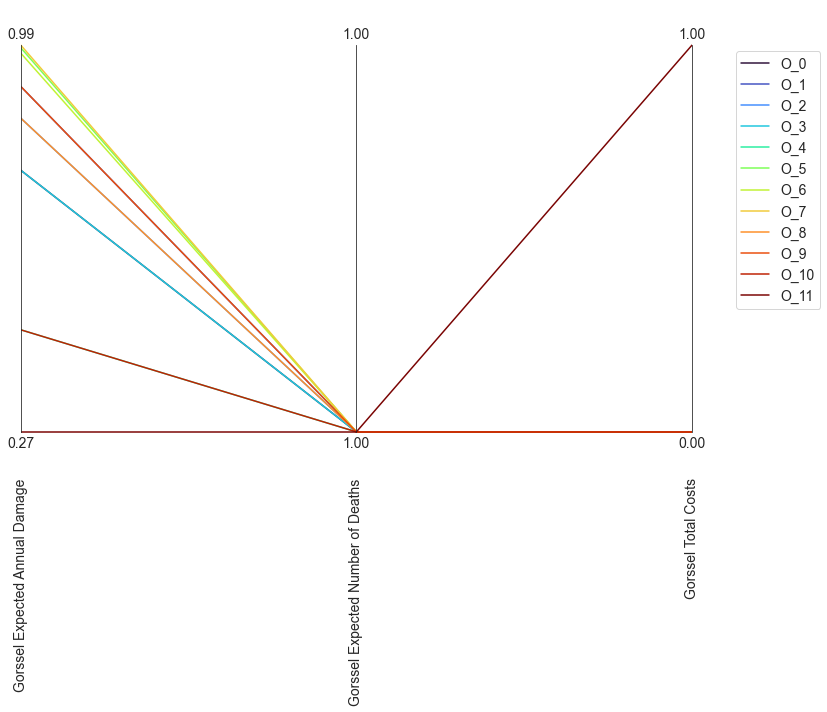
\includegraphics[width=1.15\textwidth]{report/figures/results/domain_criterion_Gorssel.png}
    \caption{Results for Gorssels domain criterion}
    \label{fig:domain_criterion_gorssel}
  \end{minipage}
  \hfill
  \begin{minipage}[b]{0.4\textwidth}
    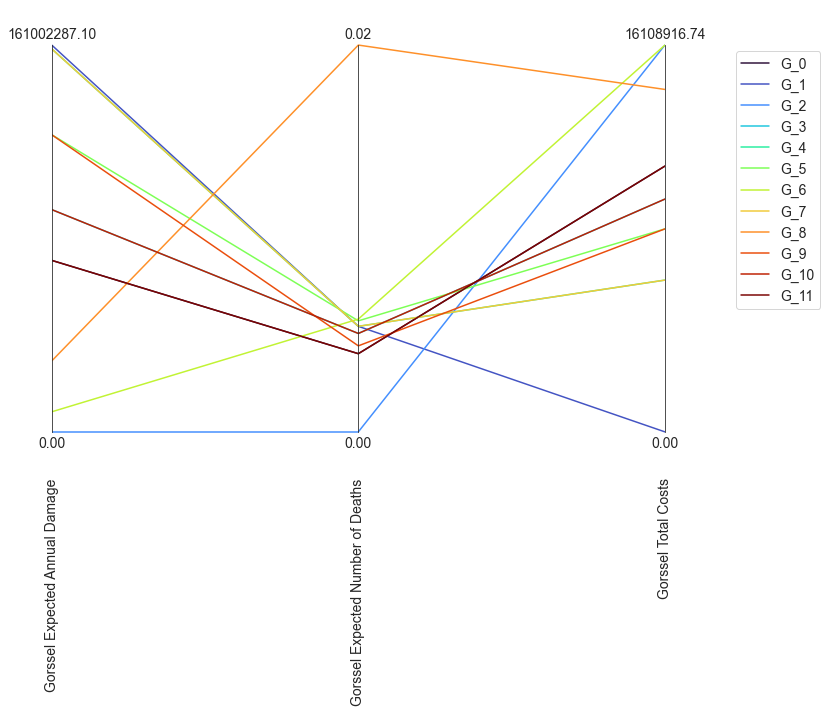
\includegraphics[width=1.15\textwidth]{report/figures/results/regret_figure_Gorssel.png}
    \caption{Results for Gorssels maximum regret}
    \label{fig:regret_gorssel}
  \end{minipage}
\end{figure}




%#################################################################
%   REGRET AND SATISFICING - DEVENTER
%#################################################################
\subsubsection{Deventer}
\textbf{results shown in figures: still have to add the tables which show the policy that is satisficing for every threshold. Also I'll put it nicely tomorrow. }
\begin{itemize}
    \item Deventer has no regret for their total costs, which is logical if they try to get Gorssel to pay for everything.
    \item Deventer has three policies that come above the now set threshold. Shown in Table \ref{tab:deventer}...
    \item Deventers results for the domain criterion show that there is only one policy solution for the best option that actually performs okay with most of the reference scenarios with a score around 0.6(damages). The other candidate-solutions score lower. 
    \item all candidate-solutions satisfy the thresholds for deventer in regards to deaths and total budget.
\end{itemize}

\begin{figure}[H]
  \centering
  \begin{minipage}[b]{0.4\textwidth}
    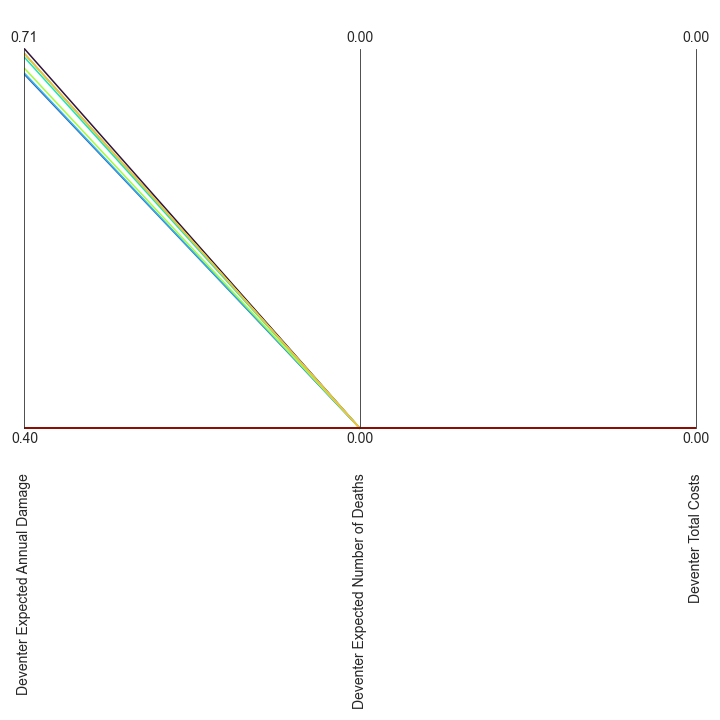
\includegraphics[width=1.15\textwidth]{report/figures/results/domain_criterion_Deventer.png}
    \caption{Results for Deventers domain criterion}
    \label{fig:domain_criterion_Deventers}
  \end{minipage}
  \hfill
  \begin{minipage}[b]{0.4\textwidth}
    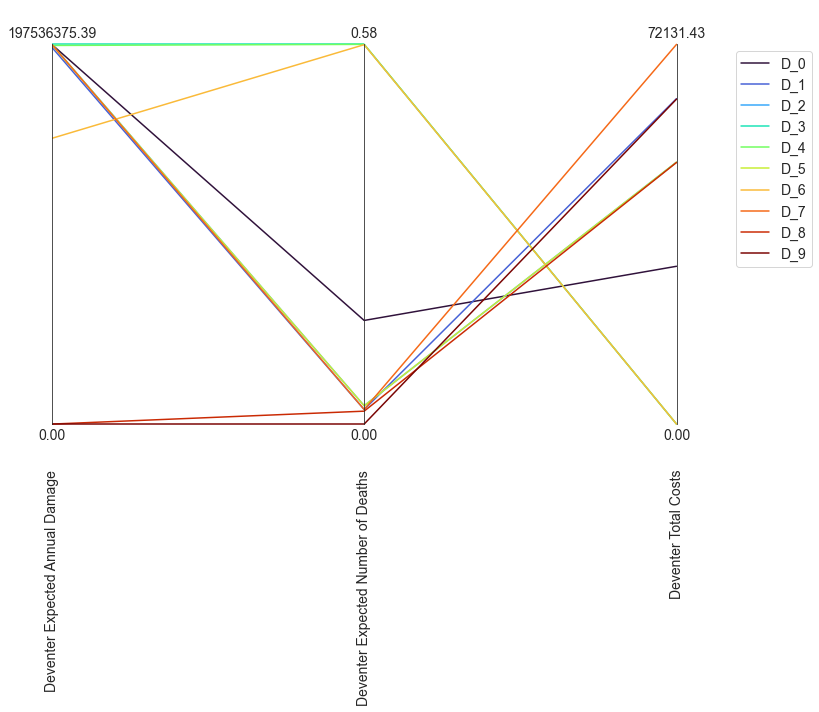
\includegraphics[width=1.15\textwidth]{report/figures/results/regret_figure_Deventer.png}
    \caption{Results for Deventers maximum regret}
    \label{fig:regret_Deventers}
  \end{minipage}
\end{figure}

%#################################################################
%   REGRET AND SATISFICING - OVERIJSSEL
%#################################################################
\subsubsection{Overijssel}
\textbf{results shown in figures: still have to add the tables which show the policy that is satisficing for every threshold. Also I'll put it nicely tomorrow. }
\begin{itemize}
    \item Overijsel has regret for their Total cost. ? or at least that is what I think the figure means.
    \item Deventer has two policies that come above the now set threshold. Shown in Table \ref{tab:deventer}...
    \item Overijssels results for the domain criterion show that there is only one policy solution for the best option that actually performs okay with most of the reference scenarios with a score around 0.6 (total costs). The other candidate-solutions score lower. 
    \item all candidate-solutions satisfy the thresholds for Overijssel in regards to deaths.
    \item for the criteria annual damage, the candiate solutions generated a wide spread of domain-criterion score. The results shown in (SHOULD I SHOW THE TABLE IN THE APPENDIX?) show that the top candidtate solutions, that fit most reference scenario's for this threshold, exist out of all possible candidate-solutions combined to their respective(base scenario?(wost/best stuff like that)
\end{itemize}
\begin{figure}[H]
  \centering
  \begin{minipage}[b]{0.4\textwidth}
    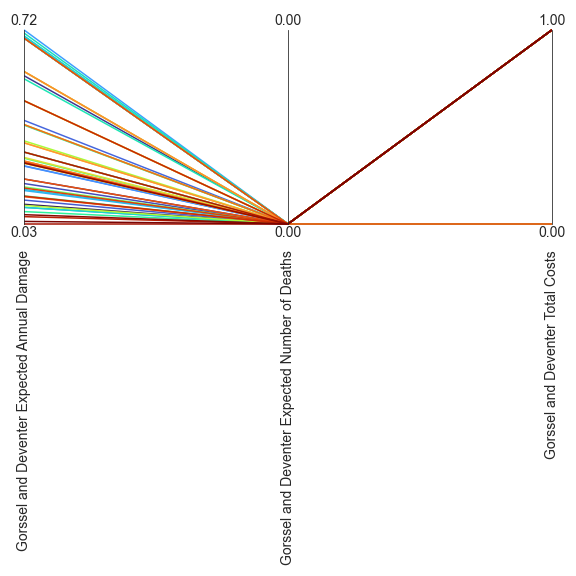
\includegraphics[width=1.15\textwidth]{report/figures/results/domain_criterion_Overijssel.png}
    \caption{Results for Overijssels domain criterion}
    \label{fig:domain_criterion_Overijssels}
  \end{minipage}
  \hfill
  \begin{minipage}[b]{0.4\textwidth}
    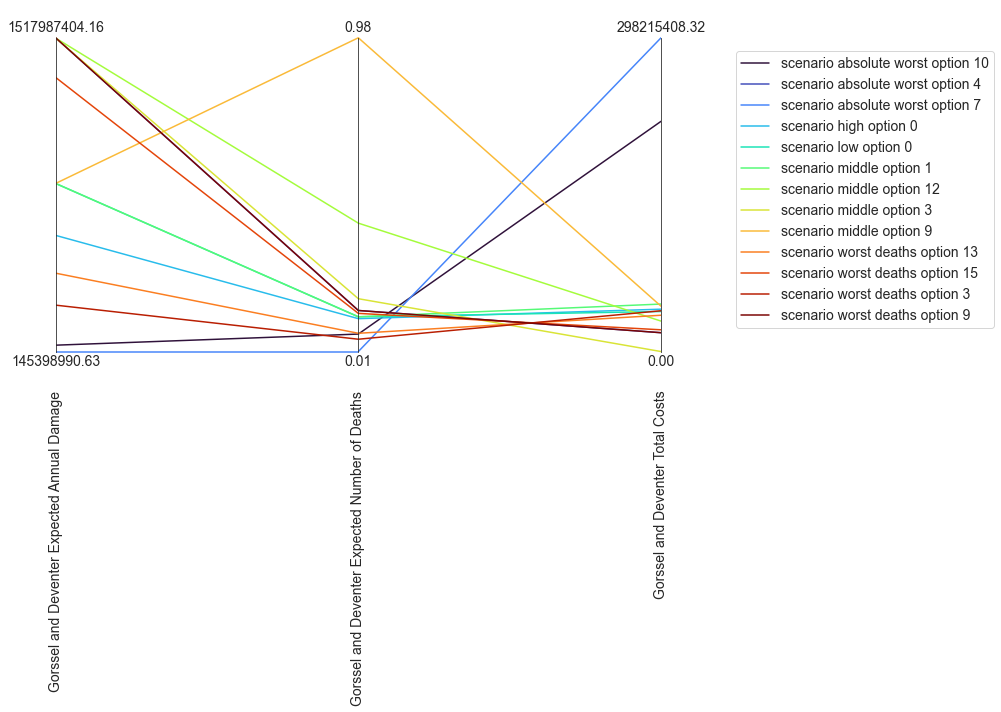
\includegraphics[width=1.15\textwidth]{report/figures/results/regret_figure_Overijssel.png}
    \caption{Results for Overijssels maximum regret}
    \label{fig:regret_Overijssels}
  \end{minipage}
\end{figure}

\subsubsection{Sensitivity Analysis}

\subsubsection{Gorssel}
\subsubsection{Deventer}
\subsubsection{Overijssel}


\subsection{Policy Comparison}
Here, the top five policies from each actor are considered and compared to investigate opportunities for coalition forming, or to identify sources of tension in the policy-making process.